% !TEX root = ./VerkListen.ja.tex

%~~~~~~~~~~~~~~~~~~~~~~~~~~~~~~~~~~~~~~~~~~~~~~~~~~~~~~~~~~~~~~~~~~~~~~~~~~~~~~~~~~~~~~~~~~~~~~~~~~~~
% Globale Definitionen für die Zeichnungen

\tikzset{node:style/.style={draw,shape=circle,thick,inner sep=1ex}}
\tikzset{node:new:style/.style={node:style,red}}
\tikzset{end:style/.style={draw,shape=rectangle}}
\tikzset{edge:style/.style={draw,thick,blue,->,shorten >=2pt}}
\tikzset{edge:new:style/.style={edge:style,red}}

\def\nodetext{\large \texttt}
\def\myXdist{1.2}

\ifthenelse{\boolean{prog_java}}{
	\def\myStartName{start}
	\def\myNullName{null}
	\def\myNullLst{\lstinline{null}}
	\def\myNodeName{node}
	\def\myNewName{newNode}
	\def\myHeadName{head}
	\def\myTailName{tail}
	\def\myMethodName{Methode}
}{}

\only<presentation>{\mode*}

\epigraph{Was eine guten Meister macht: Wissen, Können und Wollen.}{Deutsches Sprichwort}


%~~~~~~~~~~~~~~~~~~~~~~~~~~~~~~~~~~~~~~~~~~~~~~~~~~~~~~~~~~~~~~~~~~~~~~~~~~~~~~~~~~~~~~~~~~~~~~~~~~~~
\section{Datenstrukturen}
%~~~~~~~~~~~~~~~~~~~~~~~~~~~~~~~~~~~~~~~~~~~~~~~~~~~~~~~~~~~~~~~~~~~~~~~~~~~~~~~~~~~~~~~~~~~~~~~~~~~~

\begin{multicols}{2}

%----------------------------------------
\begin{frame}[fragile]
\frametitle<presentation>{Datenstrukturen}
Datenstrukturen speichern \uline{zusammengehörige Datenobjekte}.
\only<presentation>{\par}
Z.B. alle Schüler einer Klasse, alle Lieferungen an einen bestimmten Kunden.

\vspace{1ex}
\structure{\textbf{Operationen}}

Eine Datenstruktur unterstützt (meist):
\begin{itemize}
\item Einfügen
\item Entnehmen / Löschen
\item Iteration
\item Suchen
\item Anzahl
\end{itemize}

\textbf{Arrays} und \textbf{Listen} sind Datenstrukturen.
\only<article>{Eine Datenstruktur beschreibt die Art der Datenspeicherung (z.B.\ Anordnung im Speicher).}
\end{frame}
%----------------------------------------



%----------------------------------------
\begin{frame}[fragile]
\frametitle<presentation>{Listen und Arrays}

\vspace{0pt}
\begin{columns}[c]\begin{column}{0.45 \textwidth}
%...............
\structure{\textbf{Arrays}}

\begin{itemize}
\item Fixe Größe
\item Kein Hinzufügen / Löschen
\item Einfach und schnell
\end{itemize}
%...............
\end{column}\begin{column}{0.49 \textwidth}
%...............
\pause%
\structure{\textbf{Listen}}

\begin{itemize}
\item Flexible Größe
\item Einfaches Hinzufügen / Löschen
\item Ein wenig aufwendiger 
\end{itemize}
%...............
\end{column}\end{columns}
\only<presentation>{\vspace{1em}}

\pause%
Listen sind \textbf{flexibler} als Arrays und spielen in der Informatik schon sehr lange eine wichtige Rolle. 

\begin{quote}
In der \textbf{Programmiersprache LISP} (List Processor) sind Listen sogar das zentrale Element.
LISP wurde 1956 von John~McCarty entwickelt und ist bis heute in Verwendung.
\end{quote}

\end{frame}
%----------------------------------------

\end{multicols}

%~~~~~~~~~~~~~~~~~~~~~~~~~~~~~~~~~~~~~~~~~~~~~~~~~~~~~~~~~~~~~~~~~~~~~~~~~~~~~~~~~~~~~~~~~~~~~~~~~~~~
\section{Verkettete Liste}
%~~~~~~~~~~~~~~~~~~~~~~~~~~~~~~~~~~~~~~~~~~~~~~~~~~~~~~~~~~~~~~~~~~~~~~~~~~~~~~~~~~~~~~~~~~~~~~~~~~~~
\begin{multicols}{2}

%----------------------------------------
\begin{frame}<article>
\frametitle<presentation>{Verkettete Liste}

\only<presentation>{\begin{itemize}}
\only<presentation>{\item}%
Eine verkettete Liste ist eine Menge von aneinandergereihten Elementen (=\textbf{Knoten}). 
\only<presentation>{\item}%
\pause%
\begin{fact}
Bei einer verketteten Liste wird bei jedem Knoten ein Verweis auf den folgenden Knoten mit abgespeichert. 
\end{fact}
\only<presentation>{\item}%
Bei Listen sind die Knoten daher beliebig im Speicher verteilt und müssen nicht wie bei Arrays hintereinander abgespeichert sein.
\only<presentation>{\end{itemize}}

\end{frame}
%----------------------------------------

%----------------------------------------
\begin{frame}[fragile]
\frametitle<presentation>{Knoten}

\begin{definition}
Eine Liste besteht aus einzelnen \textbf{Knoten} (engl.\ node).
Ein Knoten enthält die zu speichernden Daten und den Verweis auf den \uline{nächsten} Knoten.
\end{definition}

\pause%
\structure{\textbf{Beispiel:}}

%----------------------------------------------------------------------------------------------------
\begin{center}
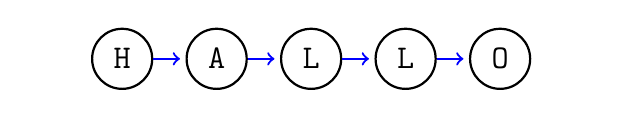
\begin{tikzpicture}
	
	\path 
		(0,0) coordinate (cs)
		++(\myXdist,0) coordinate (cv0)
		++(\myXdist,0) coordinate (cv1)
		++(\myXdist,0) coordinate (cv2)
		++(\myXdist,0) coordinate (cv3)
		++(\myXdist,0) coordinate (cv4)
		++(\myXdist,0) coordinate (ce);
	
	\path (cv0) node[node:style] (v0) {\nodetext{H}};
	\path (cv1) node[node:style] (v1) {\nodetext{A}};
	\path (cv2) node[node:style] (v2) {\nodetext{L}};
	\path (cv3) node[node:style] (v3) {\nodetext{L}};
	\path (cv4) node[node:style] (v4) {\nodetext{O}};
		
	\path[edge:style] (v0) -- (v1);
	\path[edge:style] (v1) -- (v2);
	\path[edge:style] (v2) -- (v3);
	\path[edge:style] (v3) -- (v4);
	
\end{tikzpicture}
\end{center}
%----------------------------------------------------------------------------------------

Jeder Knoten enthält hier einen Buchstaben und einen Verweis auf den folgenden Knoten.

\begin{onlyenv}<presentation>
Die Knoten können daher im Speicher durcheinander sein.
\end{onlyenv}

\end{frame}
%----------------------------------------


%----------------------------------------
\begin{frame}[fragile]
\frametitle{Implementierung}

%~~~~~~~~~~~~~~~~~~~~~~~~~~~~~~~~~~~~~~~~~~~~~~~~
\begin{assignment}{3cm}{Text}
Klasse \lstinline{Node} für einen Knoten der einen Buchstaben speichert.
\end{assignment}
\pause
\begin{vers:beamersolutions}\begin{Loesung}
\pause%
\begin{lstlisting}[emph={Node}]
public class Node {
    char data;
    Node next;
}
\end{lstlisting}
\end{Loesung}\end{vers:beamersolutions}


\end{frame}
%----------------------------------------

\end{multicols}

\pagebreak

\begin{multicols}{2}

%----------------------------------------
\begin{frame}[fragile]
\frametitle<presentation>{Anfang und Ende}
Eine Liste hat einen Anfang und ein Ende.\only<presentation>{\par}

\begin{assignment}{3cm}{Text}
Anfang und Ende einer verketteten Liste.
\end{assignment}


\begin{assignment}{3cm}{Text}
Leere Liste.
\end{assignment}


\end{frame}
%----------------------------------------


\end{multicols}

%----------------------------------------------------------------------------------------------------
\section{Listenoperationen}
%----------------------------------------------------------------------------------------------------

\begin{multicols}{2}

%----------------------------------------------------------------------------------------------------
\subsection{Eine Klasse List}

%----------------------------------------
\begin{frame}[fragile]
\frametitle<presentation>{Eine Klasse List}
\begin{assignment}{3cm}{Text}
Alle Daten und Methoden die für eine verkettete Liste notwendig sind werden in einer eigenen Klasse List zusammengefasst.
\end{assignment}

\end{frame}
%----------------------------------------



%----------------------------------------------------------------------------------------------------
\subsection{Einfügen am Anfang}

Ein neuer Knoten soll erstellt und am Anfang der Liste eingefügt werden.
%----------------------------------------
\begin{frame}[fragile]
\frametitle<presentation>{Neuer Knoten am Anfang einfügen}

\begin{assignment}{3cm}{Neuer Knoten}
Es soll ein neuer Knoten angelegt und dieser am Anfang der Liste eingefügt werden.
Skizze + Quelltext.
\end{assignment}
\pause
\begin{vers:beamersolutions}\begin{Loesung}
\pause%
\begin{lstlisting}[emph={}]
node = new Node();
node.data='L';
node.next=start;
start=node;
\end{lstlisting}
\end{Loesung}\end{vers:beamersolutions}


\end{frame}
%---------------------------------------


%----------------------------------------------------------------------------------------------------
\subsection{Liste abarbeiten}

%----------------------------------------
\begin{frame}[fragile]
\frametitle<presentation>{Liste abarbeiten}

Alle Knoten sollen "`besucht"' werden.\only<presentation>{\newline}
Zum Beispiel um alle Daten in den Knoten auszugeben.

\begin{columns}[c]\begin{column}{0.2 \textwidth}
%...............
\only<presentation>{\hfill }Anleitung:
%...............
\end{column}\begin{column}{0.7 \textwidth}
%...............
\begin{compactitem}% [<+(1)->]\addtolength{\itemsep}{-0.5\baselineskip}
\item \lstinline{Node n = start} --- Erster Knoten
\item solange weitergehen (\lstinline{n = n.next}) 
	\begin{compactitem}
	\item ... bis Ende der Liste erreicht.
	\end{compactitem}
\end{compactitem}
%...............
\end{column}\end{columns}

\begin{assignment}{3cm}{Ausgeben der Liste}
Schreibe ein Programm, das die Ausgabe aller \lstinline{data} Variablen in der verketteten Liste ermöglicht.
\end{assignment}
\pause
\begin{vers:beamersolutions}\begin{Loesung}
\pause%
\begin{lstlisting}[emph={}]
Node n=start;
while (n!=null) {
    System.out.println(n.data);
    n = n.next;
}
\end{lstlisting}
\end{Loesung}\end{vers:beamersolutions}


\end{frame}
%----------------------------------------


%----------------------------------------------------------------------------------------------------
\subsection{Erstes Element entnehmen}

%----------------------------------------
\begin{frame}[fragile]
\frametitle<presentation>{Erstes Element entnehmen}

\begin{assignment}{3cm}{Text}
Der erste Knoten soll aus der Liste entnommen werden.
Spezialfall berücksichtigen: Liste ist leer.
\end{assignment}

\end{frame}
%----------------------------------------


\end{multicols}


%----------------------------------------------------------------------------------------------------
\section{Spezialfälle}
%----------------------------------------------------------------------------------------------------

\begin{multicols}{2}
Häufiger Anwendungsfall
\begin{compactitem}
\item Ein einzelnes Datenobjekt wird gelesen
\item Das Datenobjekt wird zwischengespeichert (gemeinsam mit anderen, bereits gelesenen Datenobjekten)
\item Weitere Datenobjekte werden zwischengespeichert
\item Die zwischengespeicherten Objekte werden in einer gewissen Reihenfolge wieder entnommen.
	\begin{compactitem}
	\item Last-In / First-Out  $\rightarrow$ Stack
	\item First-In / First-Out $\rightarrow$ Queue
	\item höchste Priorität zuerst $\rightarrow$ Priority Queue
	\end{compactitem}
\item Speichern und Entnehmen kann in beliebiger Reihenfolge auftreten
\end{compactitem}

Die Datenstrukturen Stack und Queue können mit verketteten Listen implementiert werden.
Dabei finden die Einfüge und Entnahme Operationen nur am Beginn oder Ende der Liste statt.

%----------------------------------------
\begin{frame}[fragile]
\frametitle<presentation>{Spezialfälle}

\begin{onlyenv}<presentation>
Zwischenspeichern von Datenobjekten (\textit{bag abstraction})
%\vfill
\end{onlyenv}

\begin{center}
\begin{tabular}{p{3.6cm}|cc}
\textsc{} & \textsc{Stack (LiFo)} & \textsc{Queue (FiFo)} \\
\hline
Knoten einfügen                    & am Anfang & am Anfang\\
\hline
Knoten entnehmen & am Anfang & am Ende\\
\hline
{Implementierung} & {einfach} & {doppelt} \\
& {verkettete} & {verkettete} \\
& {Liste} & {Liste} \\
\hline
\end{tabular}
\end{center}

\end{frame}
%----------------------------------------

\end{multicols}


%----------------------------------------------------------------------------------------------------
\pagebreak
\section{Stack}
%----------------------------------------------------------------------------------------------------

\begin{multicols}{2}


%----------------------------------------
\begin{frame}<presentation>[fragile]
\frametitle{Stack}

(Stapel)

\begin{columns}[c]\begin{column}{0.5 \textwidth}
%...............
Operationen:
\begin{itemize}
\item \lstinline{push} --- oben auf legen
\item \lstinline{pop} --- von oben entfernen
\end{itemize}
%...............
\end{column}\begin{column}{0.5 \textwidth}
%...............
\begin{center}
\includegraphics[width=0.7\textwidth]{fig/stack01}
\end{center}
%...............
\end{column}\end{columns}

Bsp.: Stapel Bücher

\vfill
\begin{center}
Stack = LIFO (last in first out)
\end{center}
\end{frame}
%----------------------------------------

\begin{definition}
Ein Stack 
(\href{http://de.wikipedia.org/wiki/Stapelspeicher}{$\rightarrow$Link})
ist eine Datenstruktur in der Elemente einzeln hinzugefügt und entfernt werden können.
Diese beide Operationen heißen \lstinline{push} für hinzufügen und \lstinline{pop} für entfernen.
Das Verhalten ist dabei \uline{wie ein Stapel}, \lstinline{push} legt etwas oben auf und \lstinline{pop} entfernt das oberste Element (z.B.\ ein Stapel von Büchern).
\end{definition}
\begin{center}
    \includegraphics[scale=0.6]{fig/stack01}
\end{center}
Einen Stack nennt man daher auch einen LIFO (last in, first out) Speicher, weil jenes Element das zuletzt abgelegt wurde, zuerst wieder entnommen wird.

%----------------------------------------
\begin{frame}[fragile]


\begin{columns}[c]\begin{column}{0.4 \textwidth}
%...............
%~~~~~~~~~~~~~~~~~~~~~~~~~~~~~~~~~~~~~~~~~~~~~~~~
\begin{assignment}{3cm}{Text}
Zeichne den Stack der sich ergibt durch:\only<presentation>{\vspace{1em}}
\begin{addmargin}{1em}
\begin{Verbatim}
push('H')
push('e')
push('l')
push('o')
pop()
pop()
push('W')
pop()
pop()
\end{Verbatim}
\end{addmargin}

\end{assignment}
%...............
\end{column}
\begin{column}{0.6 \textwidth}
%...............
\pause
\begin{vers:beamersolutions}\begin{Loesung}
\pause%
\begin{figure}[H]
    \centering
    \includegraphics[width=0.8\textwidth]{fig/stack02}
    \caption{Stack aus Buchstaben}
\end{figure}
\end{Loesung}\end{vers:beamersolutions}
%...............
\end{column}\end{columns}

\pause
\begin{fact}
Ein Stack lässt sich sehr gut mit einer einfach verketteten Liste implementieren.
Hinzufügen und Entfernen findet am Anfang der Liste statt.
\end{fact}

\end{frame}
%----------------------------------------

%----------------------------------------
\begin{frame}[fragile]
\frametitle{Klasse für Stack}

\begin{lstlisting}[emph={}]
public class Stack {
    public void push(char c){...}
    public char pop(){...}
    public boolean empty(){...}
}
\end{lstlisting}
\pause
Zur Verwendung dieser Klasse genügt zu wissen:
\begin{compactitem}
\item Welche Methoden es gibt (push, pop, empty) und
\item wie sich diese verhalten (Stack/LIFO).
\end{compactitem}

\begin{columns}[c]\begin{column}{0.45 \textwidth}
%...............
\begin{fact}
\begin{onlyenv}<article>
Daher kann die Klasse die eigentliche Implementierung vor dem Anwender verbergen.
D.h. um diese Klasse anwenden zu können muss man nicht wissen, dass der Stack als verkettete Liste implementiert wurde.
\end{onlyenv}
Dies ist ein allgemeines Prinzip des objekt-orientierten Programmierens und wird \textbf{information hidding} (Geheimnisprinzip) genannt.
\end{fact}
%...............
\end{column}\begin{column}{0.45 \textwidth}
%...............
\begin{definition}
Welcher Teil einer Klasse öffentlich und was verborgen ist wird ausgedrückt durch:
\begin{labeling}{private~}
\item [\textsf{public}] Öffentlich
\item [\textsf{private}] Verborgen
\end{labeling}
\end{definition}
%...............
\end{column}\end{columns}



\end{frame}
%----------------------------------------


\end{multicols}

%----------------------------------------
\begin{frame}<presentation>[fragile]
\frametitle{Auswerten eines arithmetischen Ausdrucks}
%
\[3 * (2 + ( 1 + ( 7- 4) ) * (8 - 2) )\]
%
\structure{\textbf{Problem:}}
Zahlen "`merken"'.
\vfill\pause

\structure{\textbf{Dijkstra Algorithmus}}
\begin{itemize}%\addtolength{\itemsep}{-0.3\baselineskip}
\item Wert: auf Werte-Stack.
\item Operator: auf Operator-Stack.
\item \lstinline{"("} ignorieren.
\item \lstinline{")"} Operator + 2 Werte von den Stacks 
	\begin{itemize}%\addtolength{\itemsep}{-0.3\baselineskip}
	\item Ergebnis auf Werte-Stack
	\end{itemize}
\end{itemize}

\vfill
\structure{\textbf{Bsp.}}
\[(3 * (2 + 1 ) )\]

\end{frame}
%----------------------------------------

%----------------------------------------
\begin{frame}<presentation>[fragile]
\frametitle{Wie wird ein gültiger Ausdruck beschrieben?}

Gültig?
\hfill
$(3 * (2 + 1 )$
\hfill
$(3 * (2 + 1) )$
\hfill
$(3 * (2 + 1 ) + 2)$

\vfill
\structure{\textbf{Regel als Text:}} Paarweise vollständig geklammert, Zahlen nur ein Buchstabe, kein Vorzeichen

\pause\vfill
\structure{\textbf{EBNF:}} (Extended Backus-Naur Form) formal/exakt

\begin{Verbatim}
txt = "(" aus op aus ")"
aus = zf | txt
op  = "+" | "-" | "*" | "/"
zf  = "0" | "1" | "2" | "3" | "4" | "5" | "6" | "7" | "8" | "9"
\end{Verbatim}
Wenn Ausdruck mit diesen "`Produktionsregeln"' erzeugbar, dann ist er gültig.

EBNF: Syntax von Programmiersprachen
\end{frame}
%----------------------------------------

%----------------------------------------------------------------------------------------------------
\section{Queue}
%----------------------------------------------------------------------------------------------------


% Queue Operationen: offer/poll (collection Interface)
%  enqueue/dequeue - Sedgewick

\begin{multicols}{2}
%----------------------------------------
\begin{frame}[fragile]
\frametitle<presentation>{Anwendung --- Queue}

FIFO first in, first out

\begin{columns}[c]\begin{column}{0.5 \textwidth}
%...............
\includegraphics[width=0.7\linewidth]{fig/queue01.png}\par
\includegraphics[width=0.8\linewidth]{fig/queue02.png}
%...............
\end{column}\begin{column}{0.5 \textwidth}
%...............
%...............
\end{column}\end{columns}

\end{frame}
%----------------------------------------


\end{multicols}



